\documentclass[aspectratio=169]{beamer}
\usepackage[ngerman]{babel}
\usepackage{inputenc}
\usepackage[T1]{fontenc}
\usepackage{lmodern}
\usepackage{listings}
\usepackage{xcolor}
\usepackage{apacite}
\usepackage[percent]{overpic}


\bibliographystyle{apacite}


\definecolor{codegreen}{rgb}{0,0.6,0}
\definecolor{codegray}{rgb}{0.5,0.5,0.5}
\definecolor{codepurple}{rgb}{0.58,0,0.82}
\definecolor{backcolour}{rgb}{0.95,0.95,0.92}
\definecolor{TUCgreen}{cmyk}{1,0,0.9,0.2}

\lstdefinestyle{mystyle}{
    backgroundcolor=\color{backcolour},   
    commentstyle=\color{codegreen},
    keywordstyle=\color{magenta},
    numberstyle=\tiny\color{codegray},
    stringstyle=\color{codepurple},
    basicstyle=\ttfamily\footnotesize,
    breakatwhitespace=false,         
    breaklines=true,                 
    captionpos=b,                    
    keepspaces=true,                 
    numbers=left,                    
    numbersep=5pt,                  
    showspaces=false,                
    showstringspaces=false,
    showtabs=false,                  
    tabsize=2
}

\lstset{style=mystyle}

\graphicspath{{figs/}}

    \usetheme{TUC2}
  %  \usefonttheme{structureitalicserif}
    \setbeamercovered{transparent}

\newcommand{\rhomath}{\( \mathrm{\rho} \)}

\mode<presentation>
    \title{Neural Network-based Detection of Taylor Vortices in Annular Flow Systems}
    \subtitle{Exposé for Master Thesis - Initial Presentation}
    \author{\textbf{Mahyar Alikhani}}
    \institute{Institute of Applied Mechanics}
    \date{\today}

% \setbeamerfont{framesubtitle}{size=\normalfont\tiny}
%%%%%%%%%%%%%%%%%%%%%%%%%%%%%%%%%%%%%%%%%%%%%%%%%%%%%%
\begin{document}
\begin{frame}
\titlepage
% Collaborators: \footnotesize{
%   Stefan Wittek$^1$, Jendrik-Alexander Tr\"oger$^2$, Stefan Hartmann$^2$, Andreas Rausch$^1$
%      }
\end{frame}
%%%%%%%%%%%%%%%%%%%%%%%%%%%%%%%%%%%%%%%%%%%%%%%%%%%%%%

\begin{frame}
\frametitle{Contents}
\tableofcontents
\end{frame}

%%%%%%%%%%%%%%%%%%%%%%%%%%%%%%%%%%%%%%%%%%%%%%%%%%%%%%
\section{Problem Statement}
\begin{frame}
  \frametitle{Turbulent Flows and Vortices}
  \begin{itemize}
    \item Vortical formations are crucial components in the dynamics of turbulence, contributing to processes such as the generation of turbulence, amplification of mass, heat, and momentum transport.
    \item A vortex is characterized by swiriling motion of fluid around a central region.
    \item Translating this feature into a formal definition is challenging. 
  \end{itemize}
  \centering
  \textit{''A vortex exists when instantaneous streamlines mapped onto a
  plane normal to the vortex core exhibit a roughly circular or spiral
  pattern, when viewed from a reference frame moving with the
  center of the vortex core.''}
\end{frame}

%%%%%%%%%%%%%%%%%%%%%%%%%%%%%%%%%%%%%%%%%%%%%%%%%%%%%%
\subsection{Taylor-Couette flow}
\begin{frame}
  \begin{minipage}{0.45\textwidth}
    \large \color{TUCgreen}\textbf{Taylor-Couette flow}
    \begin{itemize}
      \item a Fluid dynamic phenomenon that occurs when a fluid is passing between two coaxial-rotating cylinders.
      \item Inner cylinder is typically rotating faster than outer cylinder.
      \item Dimensionless control parameters like \(\mathnormal{Re}\), $\omega_{inner}$ and $\omega_{outer}$  are key factors
    \end{itemize}
  \end{minipage}
  \begin{minipage}{0.45\textwidth}
    \vspace{-1.0 cm}
    \centering
    \begin{figure}[h]
      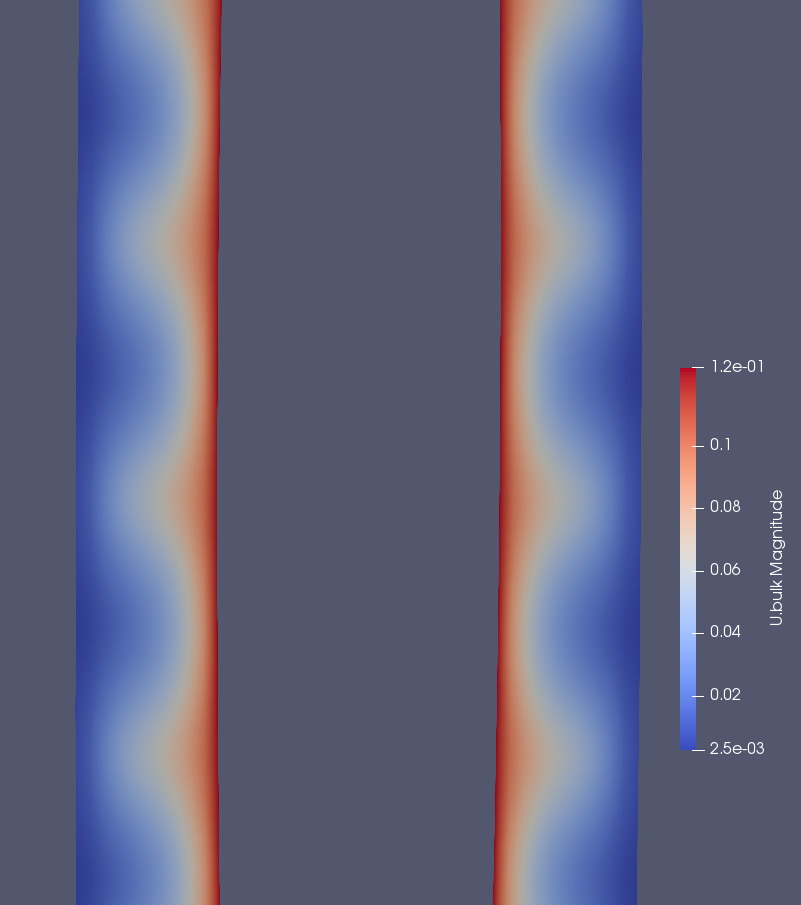
\includegraphics[width=0.9\textwidth]{Taylor_merve_vortex.png}
      \caption{\tiny{Taylor-couette flow at time-step 19}}
    \end{figure}
  \end{minipage}
\end{frame}

%%%%%%%%%%%%%%%%%%%%%%%%%%%%%%%%%%%%%%%%%%%%%%%%%%%%%%
\subsection{Vortex Detection Algorithms}
\begin{frame}
  \frametitle{Vortex Detection Algorithems}
  \begin{itemize}
  \item Vortex identificaion methods are categorized into 3 taxonomies:
    \begin{itemize}
      \item[-] \textbf{Region}/\textbf{Line}
      \item[-] \textbf{Eulerian}/\textbf{Lagrangian}.
      \item[-] \textbf{Local}/\textbf{Global}.
    \end{itemize}
    \item One of widly used algorithms is $\lambda_{2}$ method:
    \begin{itemize}
      \item  $\nabla \overline{u}$ is decomposed into \textit{symmetric}($\mathnormal{S}$) and \textit{anti-symmetric}($\mathnormal{\Omega}$) parts.
      \item three eigenvalues of $\mathnormal{S}^2+\mathnormal{\Omega}^2$ to be calculated.
      \item A point int the velocity field is a part of vortex core if at least 2 of them are negative i.e. $\lambda_{2}<0$
    \end{itemize}
  %\item Drawbacks:
  %  \begin{itemize}
  %    \item[-] may false positive be produced.
  %    \item[-] only use local operators for detecting global features.
  %  \end{itemize}
  \end{itemize}     
  
\end{frame}

%%%%%%%%%%%%%%%%%%%%%%%%%%%%%%%%%%%%%%%%%%%%%%%%%%%%%%
\section{Task definition and objective}
\begin{frame}
  \frametitle{Objectives}
  \begin{itemize}
    \item Governing equ:\\
      \begin{equation}
        \frac{\partial \mathbf{u}}{\partial t} + (\mathbf{u} \cdot \nabla)\mathbf{u} = -\frac{1}{\rho}\nabla p + \nu \nabla^2 \mathbf{u} + \mathbf{f}
      \end{equation}
    \item w.r.t boundary conditions:\\
    \begin{align}
      \mathbf{u} &= \mathbf{u}_0 \quad \text{at} \quad \Gamma_1 \\
      \mathbf{u} &= 0 \quad \text{at} \quad \Gamma_2 \\
      \frac{\partial p}{\partial n} &= 0 \quad \text{at} \quad \Gamma_3
    \end{align}

  \end{itemize}
\end{frame}
%%%%%%%%%%%%%%%%%%%%%%%%%%%%%%%%%%%%%%%%%%%%%%%%%%%%%%
\section{Litrature Review}
\begin{frame}
  \frametitle{Litrature Review}
  \begin{itemize}
    \item[(a)]  \cite{Liang2018}, a CNN-based vortex identification method to use both local and global information of flow field.
  \end{itemize}
  \begin{center}
    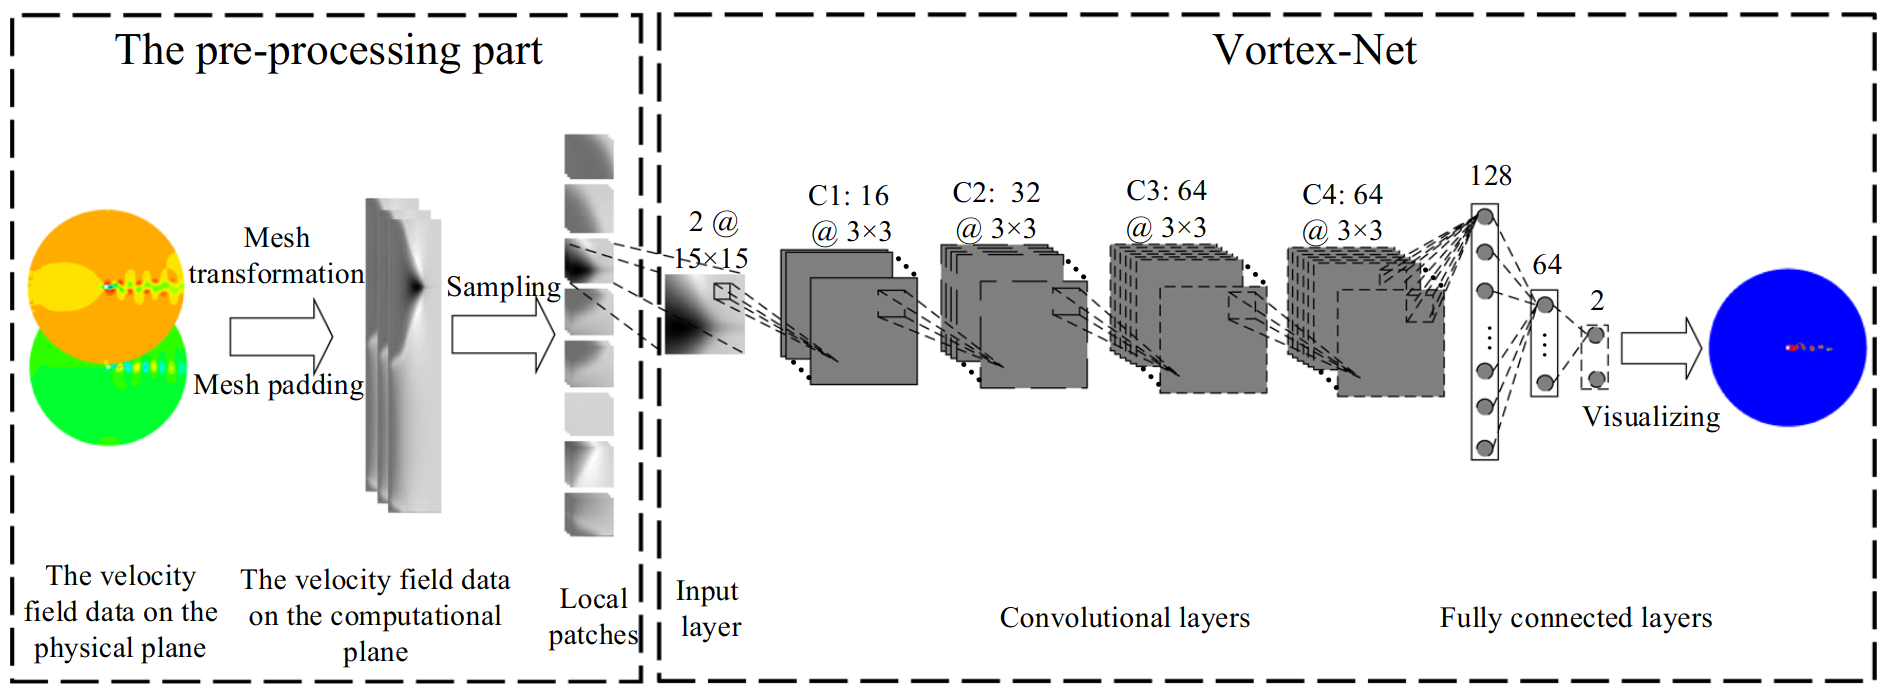
\includegraphics[width=0.85\textwidth]{paper_review.png}
  \end{center}
\end{frame}

%%%%%%%%%%%%%%%%%%%%%%%%%%%%%%%%%%%%%%%%%%%%%%%%%%%%%%
\begin{frame}
  \frametitle{Litrature Review}
  \begin{itemize}
    \item[(b)] \cite{DENG2022108229}, replacing the fully-connected NN with a segmented network to reduce the computational complexity.
  \end{itemize}
  \begin{center}
    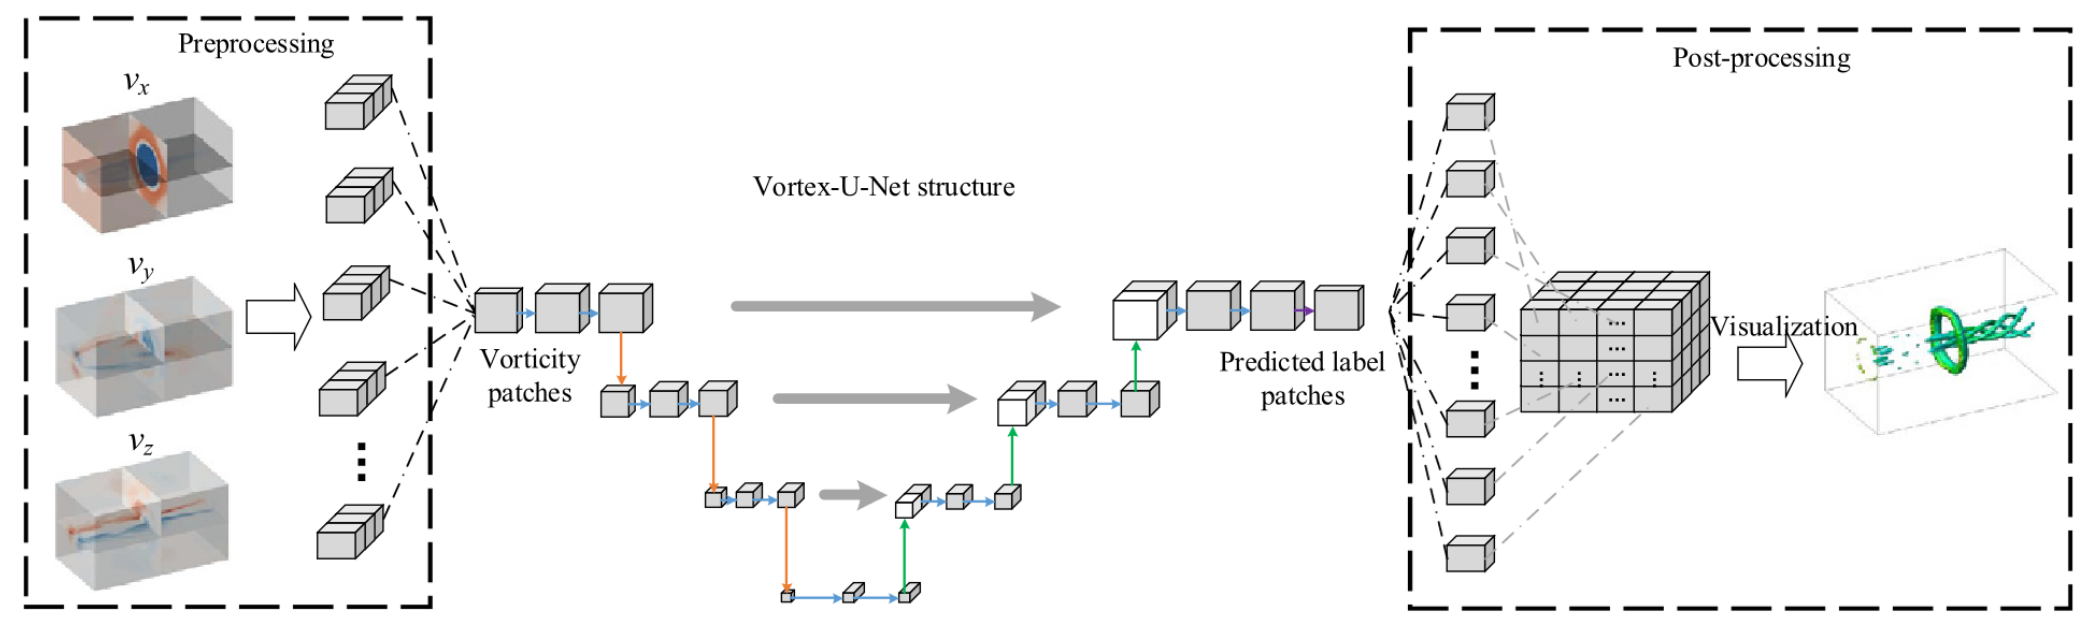
\includegraphics[width=0.9\textwidth]{U-net.png}
  \end{center}
\end{frame}

%%%%%%%%%%%%%%%%%%%%%%%%%%%%%%%%%%%%%%%%%%%%%%%%%%%%%%
\section{Approache}
\begin{frame}
  \frametitle{Approach}
  \begin{itemize}
    \item[(a)] Data preparation:
    \begin{itemize}
      \item[-] Running the  \textit{Taylor merve} case for different values of  $\{\omega_{inner}, \omega_{outer}, \mathnormal{Re}\}$
      \item[-] Collecting the velocity fields and $\lambda_2$ vectors for all time steps.
    \end{itemize}
    \item [(b)] Model development:
      \begin{itemize}
        \item Trying to Learn the mapping from a function in field to $\lambda_{2}$ method for detecting vortices.
      \end{itemize}
  \end{itemize}
\end{frame}
%%%%%%%%%%%%%%%%%%%%%%%%%%%%%%%%%%%%%%%%%%%%%%%%%%%%%%
\subsection{Deep Operator Learning (DeepOnet)}
\begin{frame}
  \frametitle{Deep operator networks\cite{lu2021learning} (DeepONets)}\
  \centering
  \begin{minipage}{0.45\textwidth}
    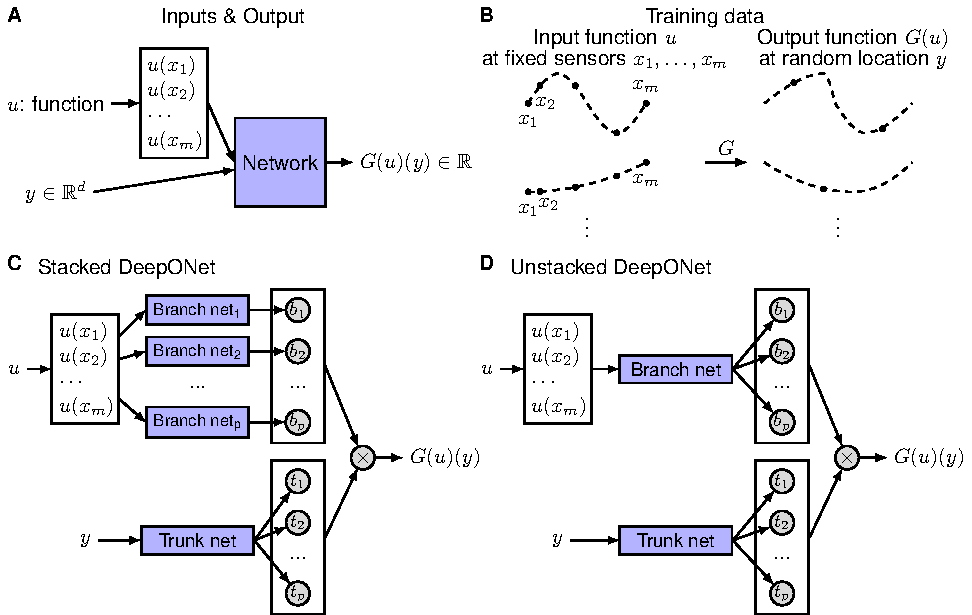
\includegraphics[width=0.8\textwidth, trim={8.12cm 0cm 0cm 0cm}, clip]{deeponet.pdf}
  \end{minipage}
  \begin{minipage}{0.45\textwidth}
    \begin{itemize}
      \item Each input function $u$ is evaluated at fixed sensor points $\{x_1, x_2, \dots, x_m\}$ 
      \item $y$ with $d$ components and $u(x_i)$ for $i = {1,2, \dots, m}$ are not matched. Therefor, it is needed to use two subnets. 
      \textbf{Branch} for encoding input function at sensor points - \textbf{Trunk} for the location to evaluate output function
    \end{itemize}
  \begin{equation}
    G(u)(y) \approx \sum_{k=1}^p b_k t_k+b_0
  \end{equation}
\end{minipage}
\end{frame}
%%%%%%%%%%%%%%%%%%%%%%%%%%%%%%%%%%%%%%%%%%%%%%%%%%%%%%
\begin{frame}
  \frametitle{Deep operator networks (DeepONets): prediction of $\lambda_2$}\
  
\begin{minipage}{0.30\textwidth}
    Inputs of branch: \\$\mathbf{u} \in \mathbb{R}^3$, ($N_s$, 3)

    Outputs of branch: \\$\boldsymbol{b} \in \mathbb{R}^{N_f}$, ($N_s$, $N_f$)

    \vspace{\baselineskip}

    Inputs of trunk: \\$\mathbf{X} \in \mathbb{R}^{128000}$, (128000, 3)

    Outputs of trunk: \\$\boldsymbol{t} \in \mathbb{R}^{N_f}$, (128000, $N_f$)
\end{minipage}
\begin{minipage}{0.30\textwidth}
    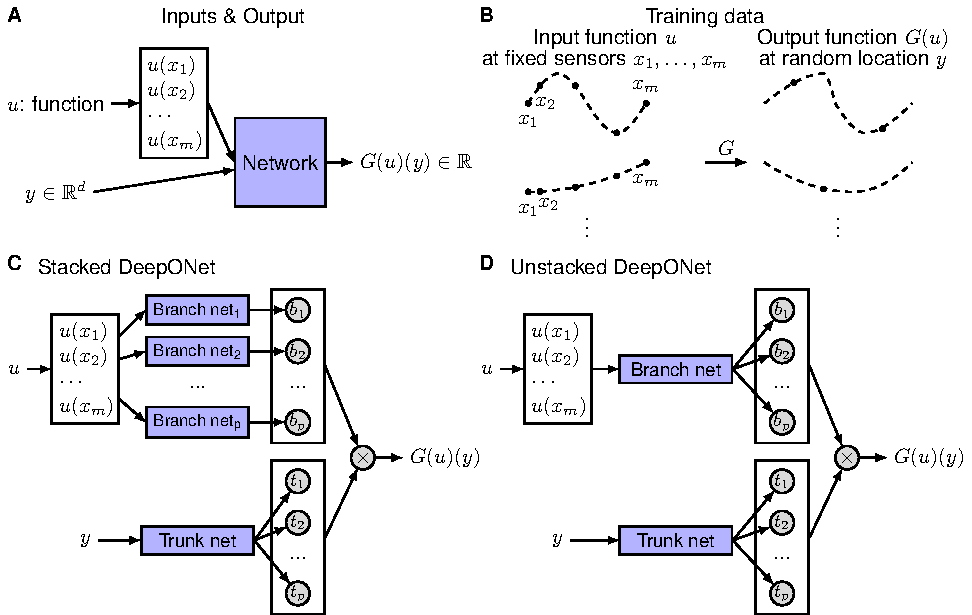
\includegraphics[width=\textwidth, trim={10.05cm 0cm 0cm 4.8cm}, clip]{deeponet.pdf}
\end{minipage}
\begin{minipage}{0.35\textwidth}

  Outputs: \\$\boldsymbol{u} \in \mathbb{R}^{1\times128000}$, \\($N_s$, $N_f$) $\bigotimes$ (128000, $N_f$)$^{T}$

\end{minipage}
\end{frame}

%%%%%%%%%%%%%%%%%%%%%%%%%%%%%%%%%%%%%%%%%%%%%%%%%%%%%%
%\begin{frame}
%\frametitle{}\
%  \begin{minipage}{0.45\textwidth}
%    \centering
%    %(A) Global ---> Global
%    \vfill
%    %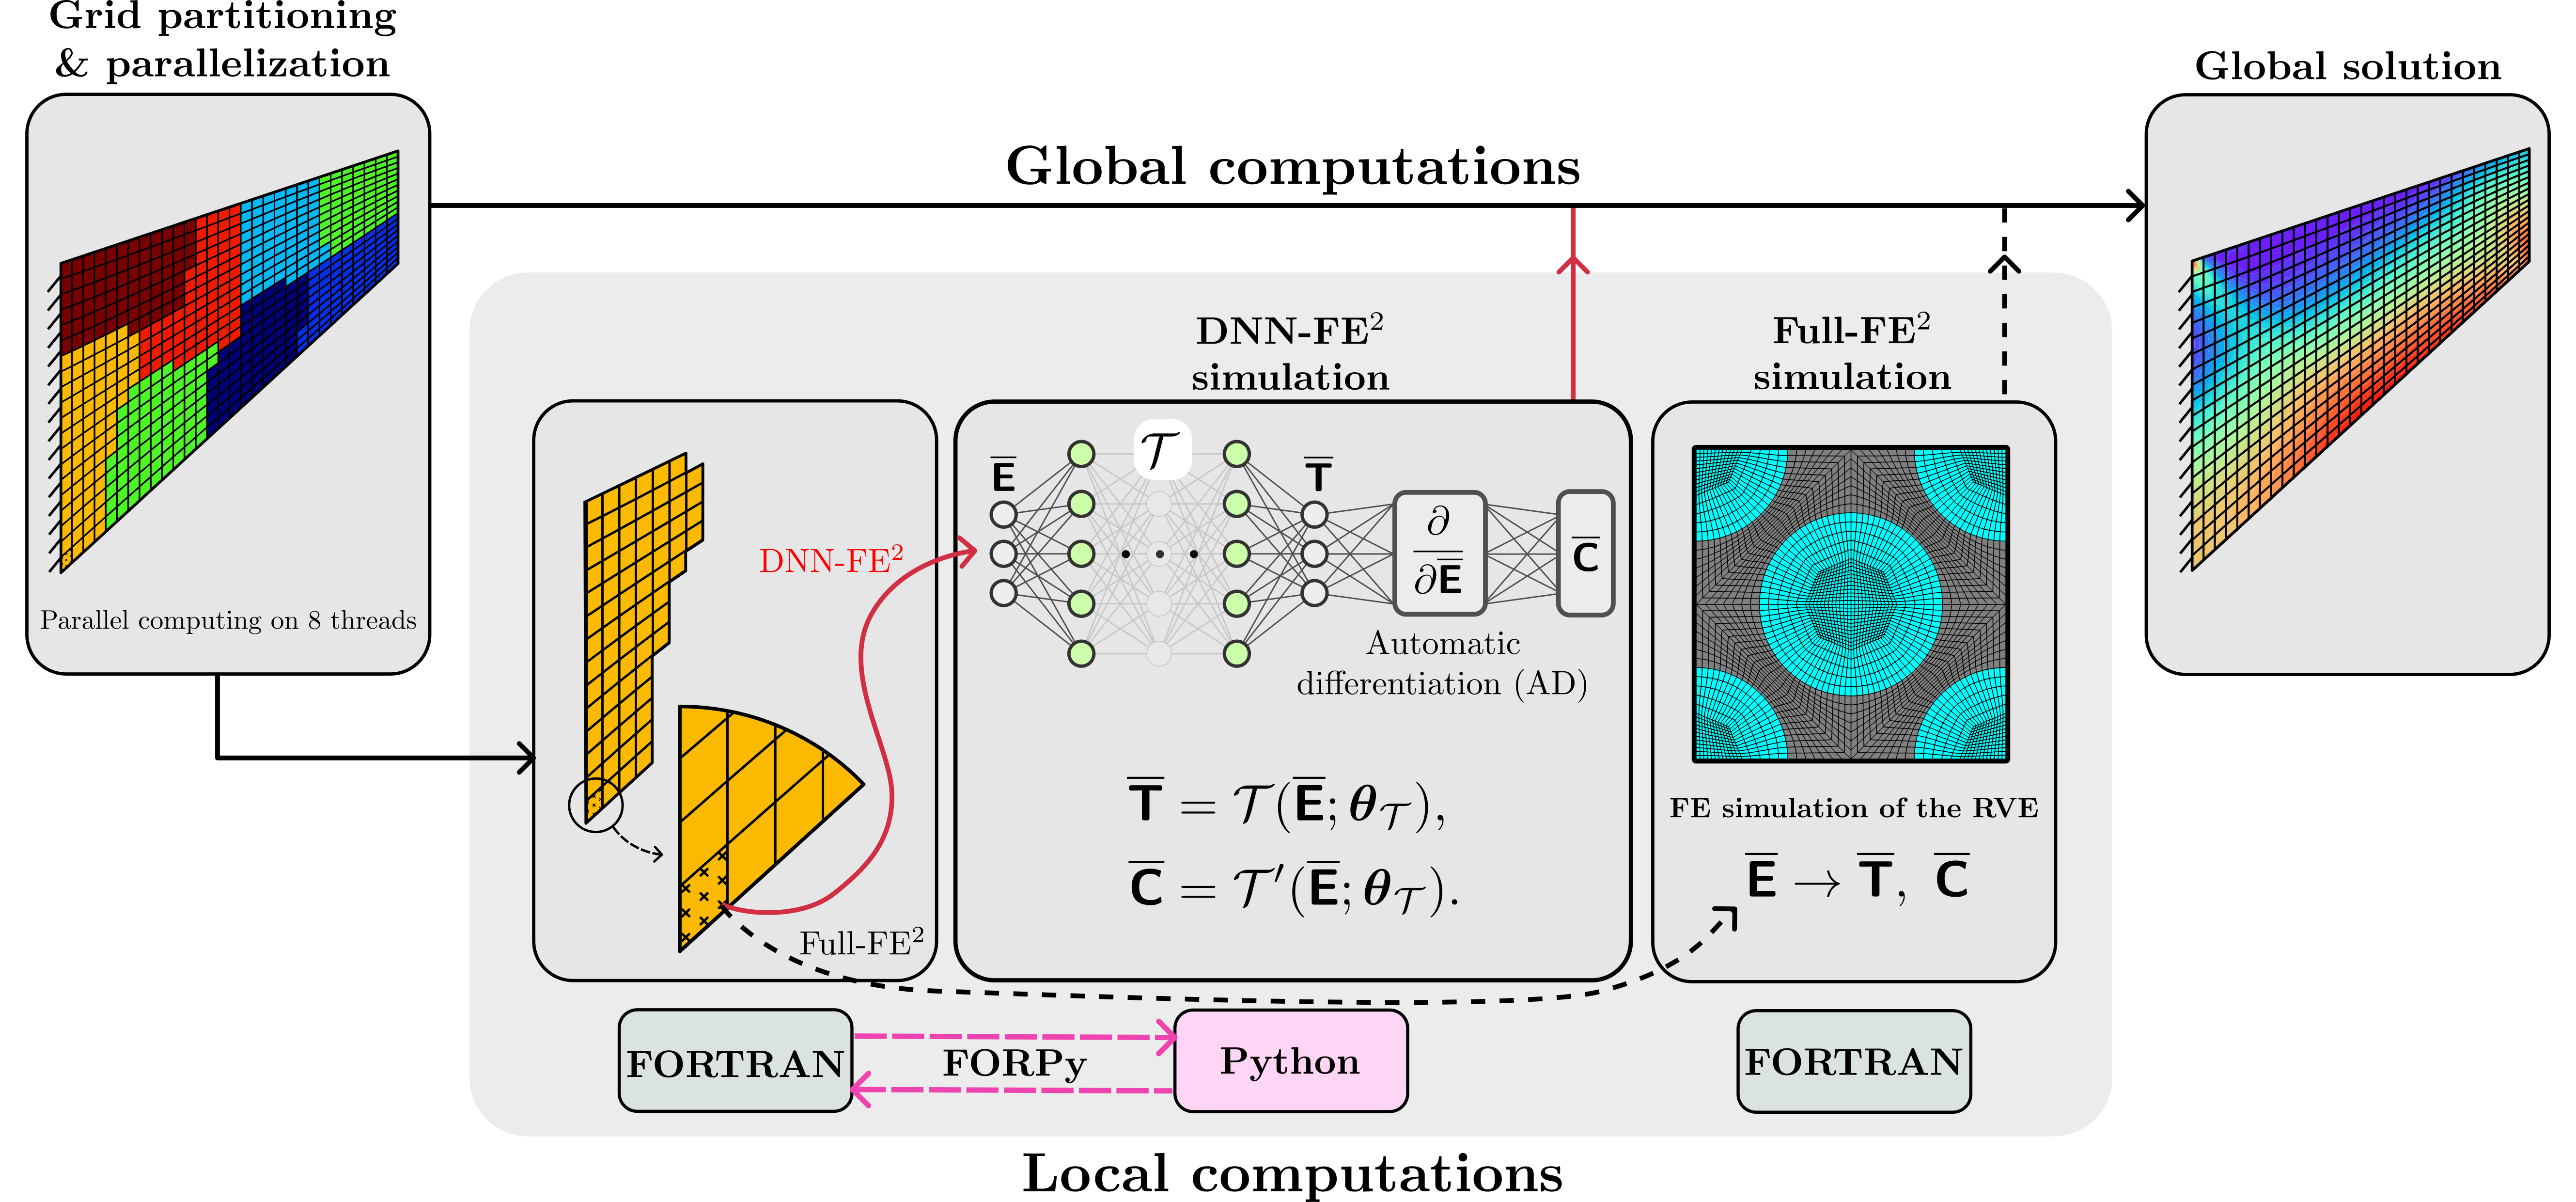
\includegraphics[width=0.9\textwidth, trim={10cm 2.3cm 9.9cm 4.2cm}, clip]{drawing}
%  \end{minipage}
%  \begin{minipage}{0.45\textwidth}
%    \centering
%    %(B) Global ---> Local ---> Global
%    \vfill
    %\hfill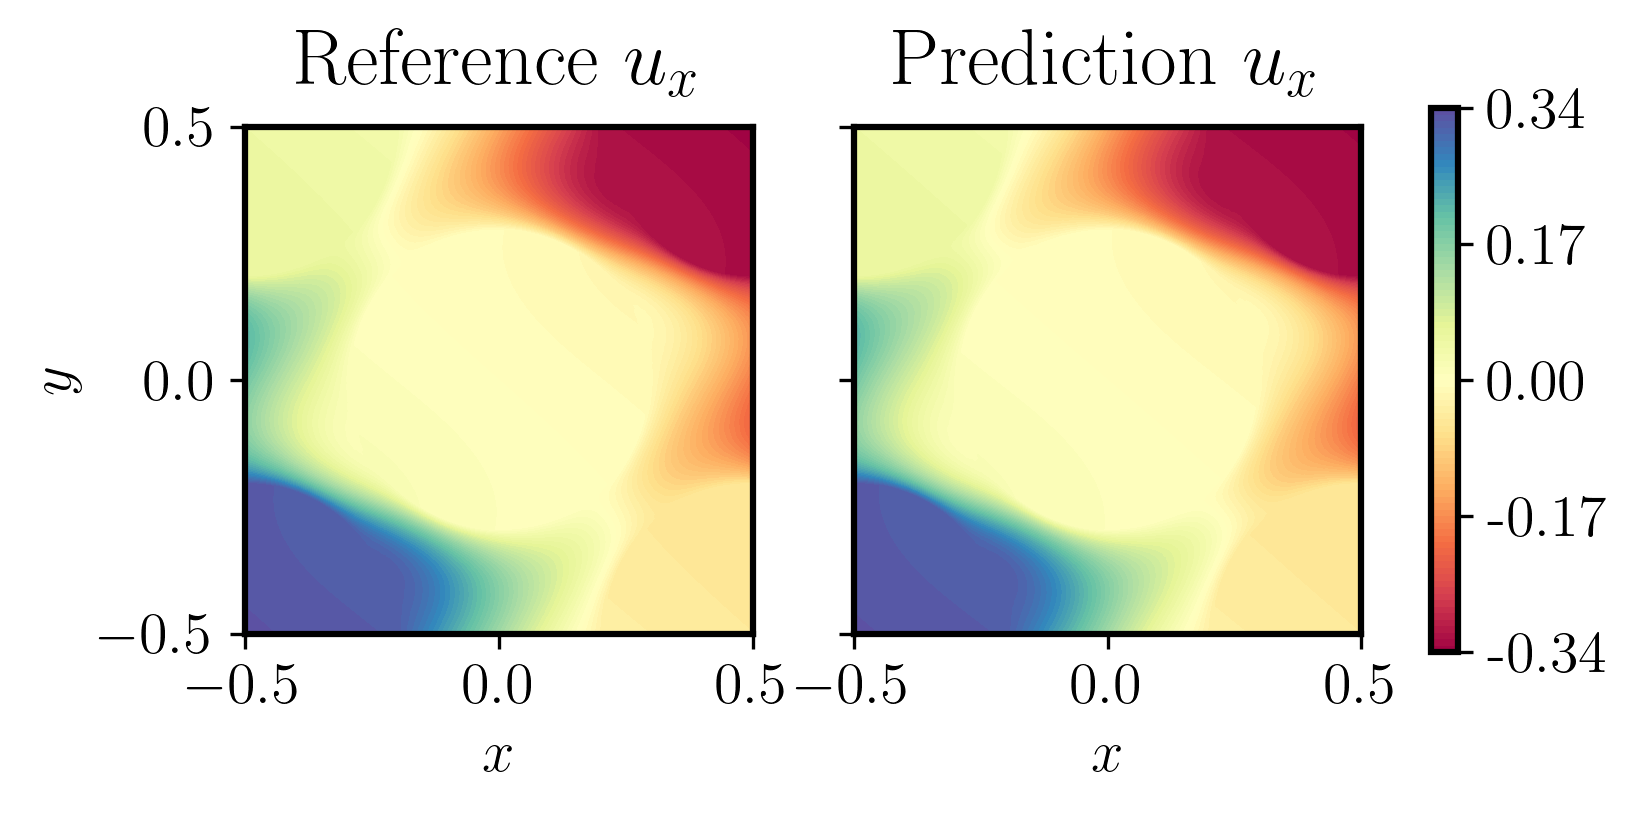
\includegraphics[width=0.95\textwidth, trim={0cm 0cm 7cm 0cm}, clip]{rve1_ux.png}
%  \end{minipage}
%\end{frame}

%%%%%%%%%%%%%%%%%%%%%%%%%%%%%%%%%%%%%%%%%%%%%%%%%%%%%%

\section{Motivation}
\begin{frame}
  \frametitle{Motivation}
  \begin{itemize}
    \item Learning the $\lambda_{2}$ operator for detecting vortices within a field.
    \item Replacing the Finit-Element mothods with NN-surrogate model
    \item Elinimate the need for manual detection of vortices in flow system using visualization 
  \end{itemize}
\end{frame}

%%%%%%%%%%%%%%%%%%%%%%%%%%%%%%%%%%%%%%%%%%%%%%%%%%%%%%

\section{Time Planning}
\begin{frame}
  \frametitle{Timeline}
  \begin{center}
    \begin{figure}
      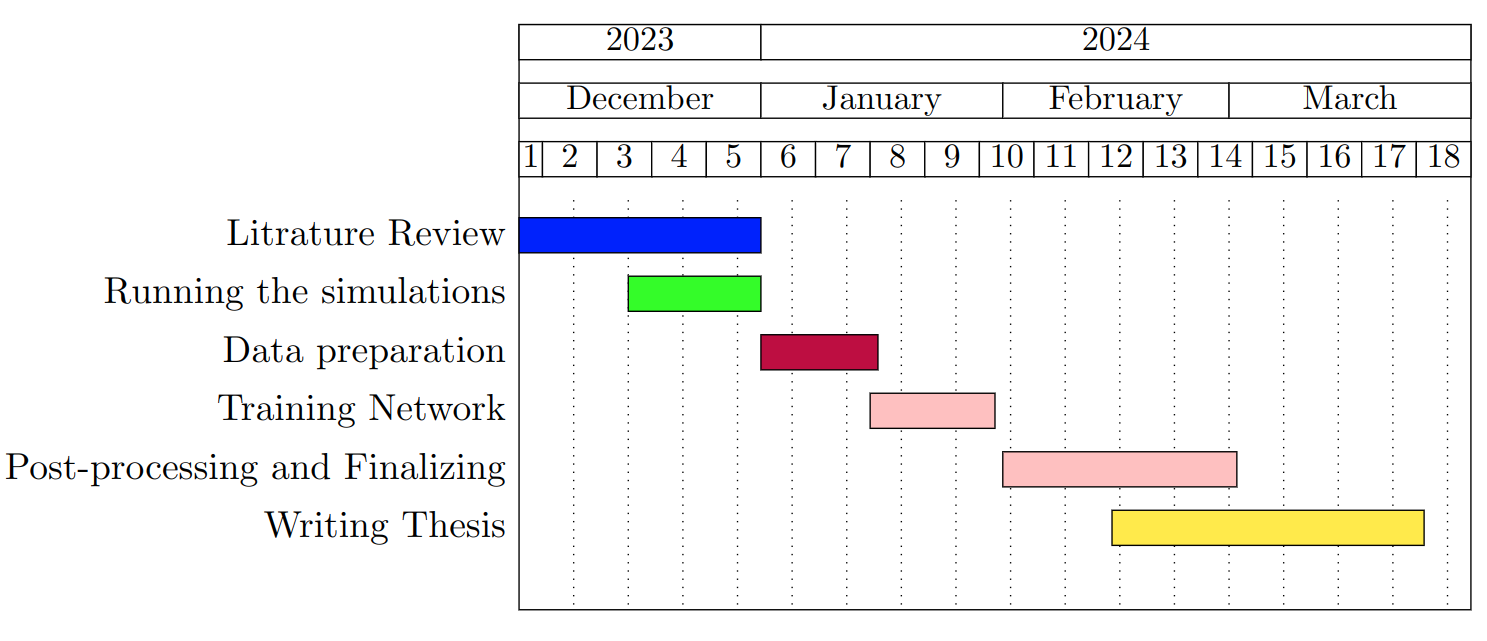
\includegraphics[width=0.9\textwidth]{figs/Timeplan.png}
      \caption{Timeplan}
    \end{figure}
  \end{center} 
\end{frame}

%%%%%%%%%%%%%%%%%%%%%%%%%%%%%%%%%%%%%%%%%%%%%%%%%%%%%%
\begin{frame}
  % \centering
  \begin{minipage}{0.1\textwidth}
    \hfill
  \end{minipage}
  \begin{minipage}{0.89\textwidth}
    \color{TUCgreen}{\textbf{\Large{Thank you!}}}\\
  \color{black}{
  \small{Any questions?}
  }
  \end{minipage}
  
\end{frame}

\bibliography{references.bib}

\end{document}

